\subsubsection{Visualization}
\label{sec:KSeMF}

To visualize the reduced \statesp\ of KS flow we will use a moving frame
to compute the first few fundamental invariants and, following the example of \CLe of \refsect{sec:CLeMF},
modify those invariants to overcome those singularities. This will help us understand what
are the invariant objects of importance in organizing the \statesp. The final goal is to choose
Poincar\'e sections that capture the dynamics but on which we can define local moving frame cross-sections, implement symmetry reduction on the Poincar\'e sections applying a moving frame on
the points of intersection of trajectories with the Poincar\'e sections and finally construct
return maps of the dynamics.

We begin by computing invariants for the ``standard action'' \refeq{eq:SO2stndrd} of $\SOn{2}$ on $\Clx{n}\cong\Rls{2n}$ which we write here as
\beq
	\left(\barr{cc} \overline{b}_k \\ \overline{c}_k\earr \right)=\left(\barr{cc}
			    			\cos(k\theta) & -\sin(k\theta)\\
						\sin(k\theta) & \cos(k\theta)\\
			   			\earr\\	
						\right) \left(\barr{cc} b_k \\ c_k\earr\right)\,,\ \ k=1,\ldots n\,.
	\label{eq:SO2stand}
\eeq
with $a_k=b_k+i c_k\,,\ b_k,c_k\in\Rls{}$.  Define the cross-section by
\beq
 	K_1(a)=c_1=0\,,
\eeq
which leads to the normalization equation
\beq
	\overline{c}_1 = \sin\theta\, b_1 +\sin\theta\, c_1 = 0\,.
	\label{eq:SO2norm}
\eeq
from which the moving frame
\beq
	\theta=-\tan^{-1}\frac{c_1}{b_1}\,.
	\label{eq:SO2stand}
\eeq
Substituting the moving frame into the rest of \refeq{eq:SO2stand} we get the fundamental invariants for the action
of $\SOn{2}$ in Fourier space of \KS\ equation. The simplifications of expressions were performed using computer algebra system Mathematica. Computation of $255$ invariants for $n=128$ took approximately $20$ minutes on a typical processor.
We list the first $11$ invariants on \reftab{tab:SO2n6}. It is important to note that computation in each irreducible
subspace (for each $k$ in \refeq{eq:SO2stand}) can be carried out independently and thus we can parallelize the computations
and also avoid recomputing invariants when increasing $n$. For the present visualization purposes, though, the  invariants
listed in \reftab{tab:SO2n6} are more than enough.

\ES{The Gr\"{o}bner basis methods usually perform poorly as $n$ becomes larger than six. On a 1GHz Pentium III processor the fundamental invariants for $n=16$, for the cross
section $b_1=0$, were computed in approximately 130s. Most importantly the time was mostly
spend in simplification of expressions.
If one only wants to project equivariant dynamics on the \reducedsp\ then the moving frame method,
through its geometric interpretation, can be used to perform the projection without explicit knowledge of the fundamental invariants.
This idea will become clear in the example of \reducedsp\ projection
for \CLe.}


\begin{table}[t]
\scriptsize
\[
\begin{array}{ll}
  u_1=r_1=\sqrt{b_1^2+c_1^2}&  \\ u_3=\frac{b_2 \left(b_1^2-c_1^2\right)+2 b_1 c_1 c_2}{r_1^2}&u_4=\frac{-2
b_1 b_2 c_1+\left(b_1^2-c_1^2\right) c_2}{r_1^2}\\ u_5=\frac{b_1 b_3 \left(b_1^2-3 c_1^2\right)-c_1 \left(-3
b_1^2+c_1^2\right) c_3}{r_1^3}&u_6=\frac{-3 b_1^2 b_3 c_1+b_3 c_1^3+b_1^3 c_3-3 b_1 c_1^2 c_3}{r_1^3}\\ u_7=\frac{b_4
\left(b_1^4-6 b_1^2 c_1^2+c_1^4\right)+4 b_1 c_1 \left(b_1^2-c_1^2\right) c_4}{r_1^4}&u_8=\frac{4 b_1
b_4 c_1 \left(-b_1^2+c_1^2\right)+\left(b_1^4-6 b_1^2 c_1^2+c_1^4\right) c_4}{r_1^4}\\ u_9=\frac{b_1
b_5 \left(b_1^4-10 b_1^2 c_1^2+5 c_1^4\right)+c_1 \left(5 b_1^4-10 b_1^2 c_1^2+c_1^4\right) c_5}{r_1^5}&u_{10}=\frac{-b_5
c_1 \left(5 b_1^4-10 b_1^2 c_1^2+c_1^4\right)+b_1 \left(b_1^4-10 b_1^2 c_1^2+5 c_1^4\right) c_5}{r_1^5}\\ u_{11}=\frac{b_6
\left(b_1^6-15 b_1^4 c_1^2+15 b_1^2 c_1^4-c_1^6\right)+2 b_1 c_1 \left(3 b_1^4-10 b_1^2 c_1^2+3 c_1^4\right) c_6}{r_1^6}&u_{12}=\frac{-2
b_1 b_6 c_1 \left(3 b_1^4-10 b_1^2 c_1^2+3 c_1^4\right)+\left(b_1^6-15 b_1^4 c_1^2+15 b_1^2 c_1^4-c_1^6\right) c_6}{r_1^6}\\
\end{array}
\]
\caption[Fundamental invariants for $\SOn{2}, n=6$]
{First $11$ fundamental invariants for the standard action
 \refneq{eq:SO2stand} of \SOn{2} on \Rls{n}.}
\label{tab:SO2n6}
\end{table}

As was the case in \CLe\ example in \refchap{chap:lasers},
there is an obvious singularity at $b_1=c_1=0$ that can be corrected by substituting
$r_1$ with $r=\sum_{i=1}^3 (b_i^2+c_i^2)$ in the denominators.
The reason for using only the first three mode magnitudes is
that dynamics in our case like to visit $\EQV{2}$ and $\EQV{3}$
and this choice is enough to prevent the denominator from
vanishing at any region of \statesp\ of dynamical interest.
With this modification one has to note that the invariants of
\reftab{tab:SO2n6} vanish at \EQB{2} and \EQB{3}. In principle
this is not a problem since we want to carry out reduction in
the principal stratum. In practice this causes two important
\eqva\ to be mapped to the origin and leads to \statesp\
portraits as in \reffig{fig:ksSO2eqbTo0}. The neighborhood of
\EQB{2} and \EQB{3} which is where we would like to get some
intuition about the behavior of \rpo s, has been squeezed into
a kink shaped structure. Inspection of the invariants in table
\reftab{tab:SO2n6} reveals
that the problem is caused by the fact that by using $c_1=0$
in the definition of the cross-section we have
assigned special importance to the first Fourier mode
which vanishes
on both \EQB{2} and \EQB{3}, causing all invariants to vanish.
We could overcome this by using the second, third, or sixth Fourier
mode to setup the moving frame but then the expressions we get after
substitution cannot be fully simplified and we loose the ability
to manipulate the denominators. We will use a higher mode to setup the moving
frame in the numerical implementation, though,
after we define suitable Poincar\'e sections.

%%%%%%%%%%%%%%%%%%%%%%%%%%%%%%%%%%%%%%%%%%%%%%%%%%%%%%%%%%%%%%%%%%
\begin{figure}[t]
\begin{center}
  (\textit{a})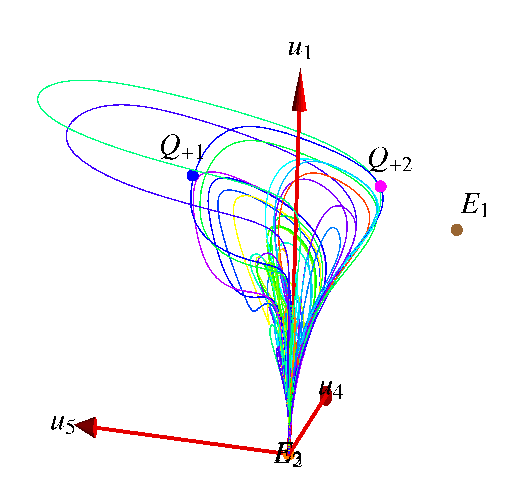
\includegraphics[width=0.4\textwidth]{../figs/ksSO2inv145eqbTo0}
\end{center}
\caption[\KS\ \SOn{2} reduced \statesp, modified invariants]
   {\Statesp\ portrait of $L=22$ \KS\ dynamics projected to
   invariants given in \reftab{tab:SO2n6}. The trajectories
   shown are 20 short \rpo s. }
\label{fig:ksSO2eqbTo0}
\end{figure}
%%%%%%%%%%%%%%%%%%%%%%%%%%%%%%%%%%%%%%%%%%%%%%%%%%%%%%%%%%%%%%%%

For visualization purposes we overcome the problem by modifying
the invariants of \reftab{tab:SO2n6} as follows. We observe
that the invariants come as either symmetric or antisymmetric
under the action of $\Dn{1}\subset\On{2}$. We modify the
symmetric invariants by adding a term $\sqrt{b_i^2+c_i^2}$
where $i$ the corresponding irreducible subspace  (Fourier
mode). The new invariants are listed in
\reftab{tab:SO2n6modif}.

\begin{table}
\begin{small}
\begin{eqnarray*}
  u_1=r_1 &=&\sqrt{b_1^2+c_1^2}\\
  u_3 &=&\frac{b_2 \left(b_1^2-c_1^2\right)+2 b_1 c_1 c_2}{r^2}\\
  u_4 &=&\sqrt{b_2^2+c_2^2}+\frac{-2
b_1 b_2 c_1+\left(b_1^2-c_1^2\right) c_2}{r^2}\\
  u_5 &=&\sqrt{b_3^2+c_3^2}+\frac{b_1 b_3 \left(b_1^2-3 c_1^2\right)-c_1 \left(-3
b_1^2+c_1^2\right) c_3}{r^3}\\
  u_6 &=&\frac{-3 b_1^2 b_3 c_1+b_3 c_1^3+b_1^3 c_3-3 b_1 c_1^2 c_3}{r^3}\\
  u_7 &=&\frac{b_4
\left(b_1^4-6 b_1^2 c_1^2+c_1^4\right)+4 b_1 c_1 \left(b_1^2-c_1^2\right) c_4}{r^4}\\
  u_8 &=&\sqrt{b_4^2+c_4^2}+\frac{4 b_1
b_4 c_1 \left(-b_1^2+c_1^2\right)+\left(b_1^4-6 b_1^2 c_1^2+c_1^4\right) c_4}{r^4}\\
  u_9 &=&\sqrt{b_5^2+c_5^2}+\frac{b_1
b_5 \left(b_1^4-10 b_1^2 c_1^2+5 c_1^4\right)+c_1 \left(5 b_1^4-10 b_1^2 c_1^2+c_1^4\right) c_5}{r^5}\\
  u_{10} &=&\frac{-b_5
c_1 \left(5 b_1^4-10 b_1^2 c_1^2+c_1^4\right)+b_1 \left(b_1^4-10 b_1^2 c_1^2+5 c_1^4\right) c_5}{r^5}\\
  u_{11} &=&\frac{b_6
\left(b_1^6-15 b_1^4 c_1^2+15 b_1^2 c_1^4-c_1^6\right)+2 b_1 c_1 \left(3 b_1^4-10 b_1^2 c_1^2+3 c_1^4\right) c_6}{r^6} \\
  u_{12} &=&\sqrt{b_6^2+c_6^2}+\frac{-2
b_1 b_6 c_1 \left(3 b_1^4-10 b_1^2 c_1^2+3 c_1^4\right)+\left(b_1^6-15 b_1^4 c_1^2+15 b_1^2 c_1^4-c_1^6\right) c_6}{r^6}
\end{eqnarray*}
\caption[Modified invariants for $\SOn{2}, n=6$]
{Modified invariants for the standard action of \SOn{2} on \Rls{6}}
\label{tab:SO2n6modif}
\end{small}
\end{table}

\Statesp\ projections on those invariants are shown in
\reffig{fig:SO2inv}\ES{Sophia says: Do not scrible-scrable!}.
\ES{Those projections make me feel desperate. My only hope is
that the unstable manifolds of the \reqva\ and the
unstable manifolds of the antisymmetric \eqva\ that are not
restricted in the antisymmetric subspace (and we haven't payed
any attention to) will play some role in organizing this mess.}
Visualizing the unstable manifold of $\REQV{\pm}{1}$ is not a
straightforward task, since it is $4$-dimensional, see \reftab{tab:Eksym}.
Nevertheless, we can get an idea of its importance for the dynamics
by plotting the continuation of the $\eigExp[1,2]$ eigenplane under the flow,
see \reffig{fig:SO2inv}.
We observe that even though the neighborhood of \REQV{\pm}{1} is not visited
by the ``turbulent'' dynamics or the \rpo s, the unstable manifold
of \REQV{\pm}{1} potentially plays an important role in organizing the flow, a situation
that we have also encountered in Lorenz and \CLe examples.
The same is true for the trajectories originating in the $\eigExp[1,2]$ eigenspace of \EQV{1}
that are not in the antisymmetric subspace. Of course those observations
are at this point of a rather speculative character as projections are frequently
misleading. We will only be able to verify those statements after we reduce
the dynamics to discrete time maps on suitable Poincar\'e sections,
see \refchap{chap:tobedone}.



%%%%%%%%%%%%%%%%%%%%%%%%%%%%%%%%%%%%%%%%%%%%%%%%%%%%%%%%%%%%%%%%%%
\begin{figure}[t]
\begin{center}
  (\textit{a})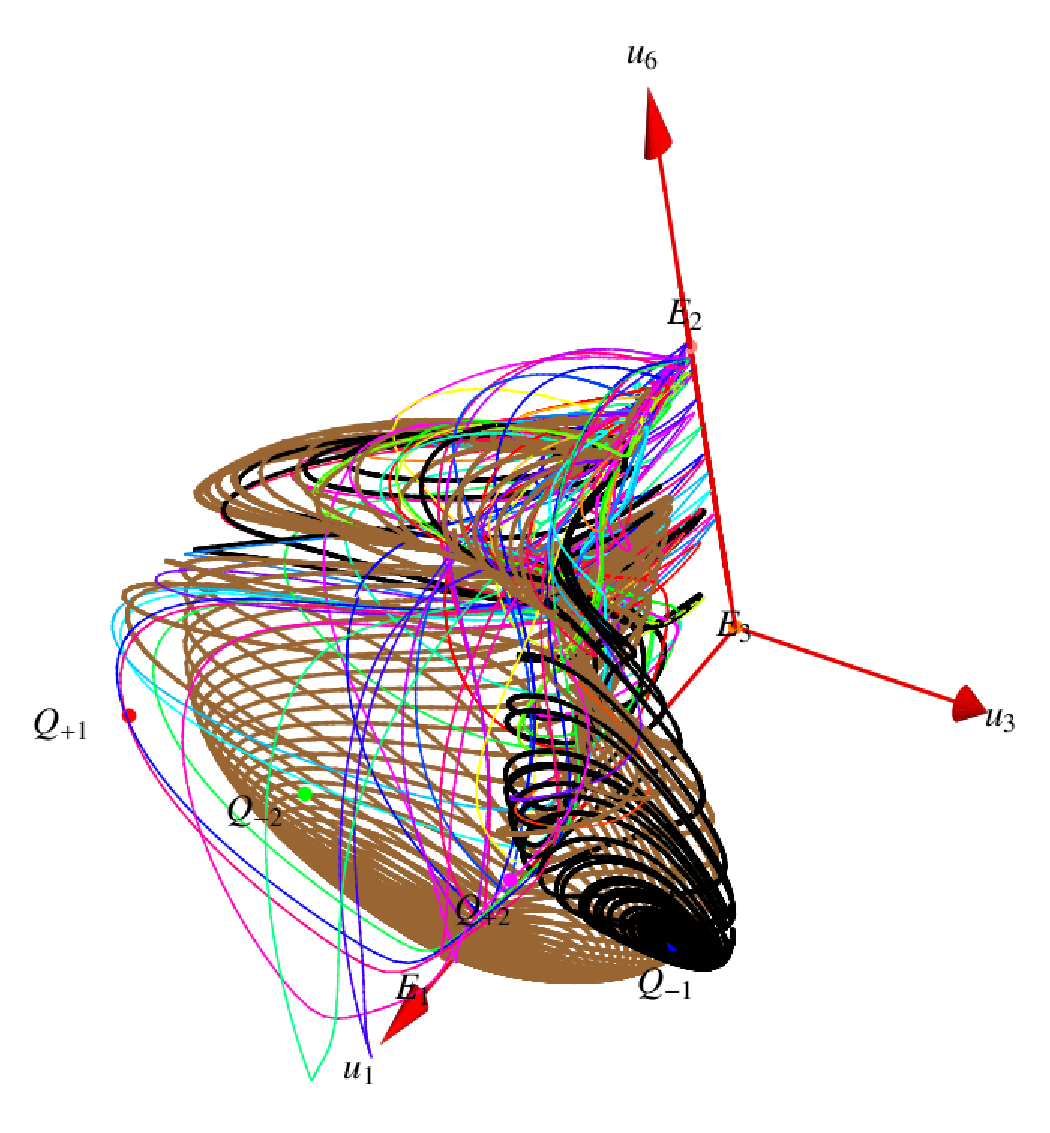
\includegraphics[width=0.45\textwidth]{../figs/ksSO2inv134}
~~~~(\textit{b})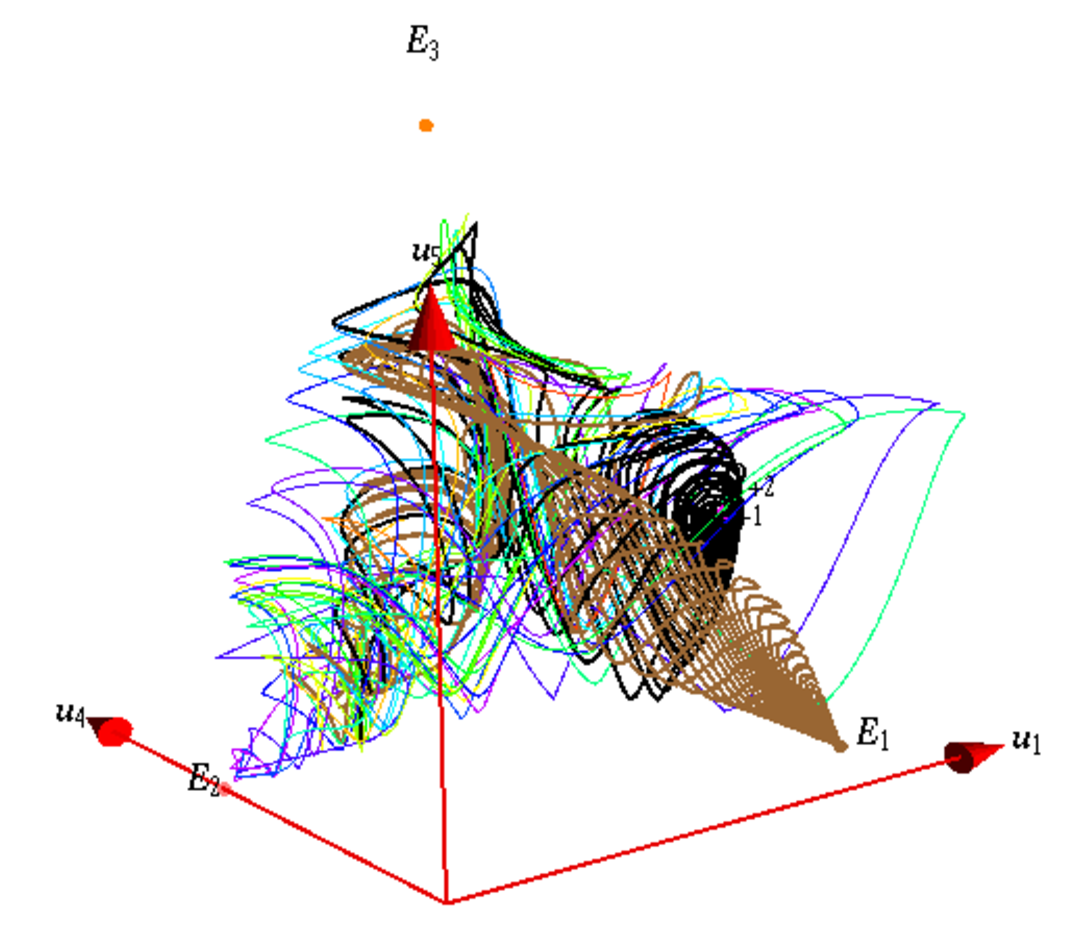
\includegraphics[width=0.45\textwidth]{../figs/ksSO2inv145}
\end{center}
\caption[\KS\ \SOn{2} reduced \statesp\ projection II]
{Two different projections of L=22 \KS\ dynamics on invariants
given in \reftab{tab:SO2n6modif}. Shown are 20
short \rpo s. Part of the unstable manifold of
$\REQV{-}{1}$ is shown in black and part of the unstable manifold of $\EQV{1}$ is
shown in brown.}
\label{fig:SO2inv}
\end{figure}
%%%%%%%%%%%%%%%%%%%%%%%%%%%%%%%%%%%%%%%%%%%%%%%%%%%%%%%%%%%%%%%%
